\documentclass[journal]{IEEEtran}
\usepackage[T1]{fontenc}
\usepackage{amsmath,amssymb}
\usepackage{booktabs,array,graphicx}
\usepackage{cite}
\usepackage{access-layout}
\usepackage{tikz}
\usetikzlibrary{arrows.meta,positioning,fit}
\usepackage[hidelinks]{hyperref}
\hypersetup{pdftitle={AegisHealth: An Agentic AI Framework for Explainable and Evidence-Grounded Clinical Decision Support}}
\newcommand{\system}{AegisHealth}
\begin{document}
\special{papersize=8in,10.875in}
% Author identities and affiliations omitted until supplied.
\twocolumn[{
\begin{minipage}{\textwidth}
\vspace{4mm}
{\color{accessblue}\sffamily\fontsize{22}{26}\selectfont\raggedright
AegisHealth: An Agentic AI Framework for Explainable and Evidence-Grounded Clinical Decision Support\par}
\vspace{6mm}
\begin{abstract}
Clinical decision support requires more than a predictive probability: users must understand the measurements influencing an estimate and inspect the evidence supporting its interpretation. This paper presents AegisHealth, a modular agentic framework combining cardiovascular disease classification, Shapley Additive Explanations, and retrieval augmented generation within a React dashboard and FastAPI service. The implementation uses the Cleveland subset of the UCI Heart Disease dataset, comprising 303 records and thirteen predictors. Nine prespecified classifier configurations are compared using repeated stratified cross validation on 242 development records, with preprocessing fitted separately inside each training fold. Regularized logistic regression is selected and evaluated on 61 held out records, achieving accuracy of 88.52 percent and ROC AUC of 0.9610. Probability scale explanations identify influential original features, which guide semantic retrieval from a versioned local index of the 2019 ACC/AHA prevention guideline executive summary. Retrieved passages retain source provenance and support optional, constrained cloud language model synthesis. Six development queries yield mean Precision@2 of 0.5833, revealing retrieval failures. Experiments do not establish clinician benefit, hallucination reduction, or complete cloud response latency. The contribution is an auditable implementation linking prediction, attribution, and evidence while exposing uncertainty, partial execution, and the limitations of historical diagnostic data for clinical deployment.
\end{abstract}
\begin{IEEEkeywords}
Agentic AI, clinical decision support, explainable AI, retrieval-augmented generation, cardiovascular disease.
\end{IEEEkeywords}
\end{minipage}
\vspace{7mm}
}]

\section{Introduction}
Clinical decision-support systems (CDSS) often present the output of a supervised predictor as a score or binary classification. Cardiovascular prediction studies demonstrate the utility of machine learning for organizing structured clinical measurements, including hybrid approaches reported in IEEE Access~\cite{mohan2019}. However, predictive discrimination, explanation, and clinical justification are different requirements. A model may distinguish historical labels while offering little support for interpreting a particular prediction or verifying whether a recommendation applies to the patient under review.

Post hoc feature attribution addresses part of this problem by describing how inputs influence model output. SHapley Additive exPlanations (SHAP) provides a principled additive attribution framework~\cite{lundberg2017}. Nevertheless, an explanation of a fitted predictor is not proof of causal relevance or clinical correctness. Rudin argues for inherently interpretable models in high-stakes applications~\cite{rudin2019}; Ghassemi \emph{et al.} further challenge the assumption that current explanation methods alone establish trustworthiness in healthcare~\cite{ghassemi2021}. These observations motivate an explicit separation between a numerical explanation and the medical evidence consulted when communicating that explanation.

Retrieval-augmented generation (RAG) supplies a complementary mechanism: external passages are retrieved and provided to a language model, rather than relying exclusively on its parametric memory~\cite{lewis2020}. Medical RAG benchmarks demonstrate that corpus, retrieval, and generator choices materially affect question-answering performance~\cite{xiong2024}. Multi-agent medical reasoning has also been studied using collaborating language-model roles~\cite{tang2024}. Consequently, this work does not claim that clinical agents or medical RAG are new. Its narrower engineering question is whether a reproducible structured-data pipeline can expose prediction, local attribution, evidence provenance, and synthesis status through one coherent interface.

\system{} addresses this question using five functional responsibilities: data processing, prediction, explainability, medical knowledge retrieval, and recommendation synthesis. These responsibilities are orchestrated in a centralized application; they are not five autonomous language models or independently deployed services. The current implementation deliberately selects its classifier from measured development performance, rather than assuming that a boosted tree must be preferable.

The contributions are: (i) a reproducible comparison of nine classifier configurations with a protected holdout; (ii) original-feature, probability-scale SHAP connected to versioned guideline retrieval; and (iii) an application contract that preserves useful local results when cloud synthesis is unavailable. The evaluation reports both favorable predictive results and retrieval failures. The target is \emph{existing disease presence in the historical Cleveland cohort}, not prospective cardiovascular risk, a validated diagnosis, or a ten-year ASCVD score. This distinction is essential because the retrieved document concerns primary prevention, whereas several model inputs arise from diagnostic investigations.

\section{Related Works}
\subsection{Machine Learning for Disease Prediction}
Mohan \emph{et al.} investigate hybrid machine-learning techniques for heart-disease prediction~\cite{mohan2019}. Such work motivates comparative classification experiments, but reported scores cannot be compared directly across different data cleaning rules, splits, feature encodings, and evaluation protocols. Chen and Guestrin introduce XGBoost as a scalable regularized tree-boosting system~\cite{chen2016}. It is an appropriate candidate for heterogeneous tabular predictors, although algorithmic sophistication does not guarantee the best performance on a small clinical dataset.

In \system{}, regularized logistic regression is retained because it has the highest mean development ROC-AUC among the tested configurations. This choice is compatible with the argument that an interpretable model should not be discarded merely because a more complex alternative is available~\cite{rudin2019}. The comparison is bounded by the prespecified settings: it does not establish a universally optimal classifier, nor does it reproduce another study's protocol.

\subsection{Explainable AI in Clinical Settings}
Lundberg and Lee unify additive feature-attribution methods and formalize desirable explanatory properties~\cite{lundberg2017}. A feature contribution answers a model-specific question about the change in output associated with that feature under a defined background distribution. It does not establish that altering the feature would change a patient's outcome. Moreover, correlated predictors and the choice of background data affect the interpretation of masking-based explanations.

Ghassemi \emph{et al.} caution against treating explanation interfaces as substitutes for rigorous clinical validation~\cite{ghassemi2021}. Accordingly, \system{} displays signed contributions and source evidence separately, marks missing inputs, and avoids presenting a contribution as a treatment recommendation. The implemented permutation explainer operates on the complete preprocessing--classification pipeline, preserving the original thirteen feature groups rather than independently masking one-hot columns.

\subsection{Language Models, Retrieval, and Medical Agents}
Lewis \emph{et al.} establish a RAG formulation combining parametric generation with nonparametric document memory~\cite{lewis2020}. \system{} adopts the retrieve-then-generate pattern, but does not jointly train a retriever and generator. Its retrieval encoder, classifier, and cloud generator remain separately configured components.

Xiong \emph{et al.} introduce MIRAGE and the MedRAG toolkit to evaluate medical question answering across corpora, retrievers, and language models~\cite{xiong2024}. Their findings support measuring retrieval quality independently of generation fluency. Tang \emph{et al.}'s MedAgents uses expert-role analyses, summarization, and iterative discussion for medical reasoning~\cite{tang2024}. In contrast, \system{} uses a fixed dependency graph and one optional generation call. It neither implements multi-round deliberation nor claims the capabilities reported on those question-answering benchmarks.

A monolithic application can also be interpretable and evidence-grounded; modularity alone does not guarantee either property. The practical advantage sought here is explicit intermediate contracts: errors can be localized to prediction, attribution, retrieval, or synthesis, and a failed component need not erase valid upstream results. The corresponding costs include coordination logic, additional failure states, and latency across dependent stages. No ablation against a monolithic baseline has been performed.

\section{Proposed Methodology}
\subsection{System Architecture and Functional Agents}
The repository combines a React/TypeScript/Vite frontend with a FastAPI backend. The dashboard uses shadcn components and Recharts to present patient measurements, disease probability, signed feature contributions, guideline excerpts, and an optional summary. Markdown tables and citation markup are rendered through a sanitized pipeline; exact source text remains available for inspection. Editing patient values invalidates previous results, reducing the chance that stale output is mistaken for a new assessment.

The five functional agents map to concrete implementation responsibilities:
\begin{enumerate}
\item \textbf{Data Processing Agent:} typed API validation checks feature names, numerical ranges, and original UCI category codes. A saved preprocessing pipeline applies training-derived imputation, scaling, and encoding; it is not refitted during inference.
\item \textbf{Prediction Agent:} the saved scikit-learn pipeline estimates positive-class probability using the selected logistic classifier. Prediction is invoked inside the explanation service rather than exposed as an independent network agent.
\item \textbf{Explainability Agent:} \texttt{PatientExplainer} computes permutation SHAP, verifies probability additivity, and ranks original features by absolute contribution.
\item \textbf{Medical Knowledge Agent:} The retriever embeds an attribution-derived query and searches a persistent Chroma collection for two guideline passages with provenance.
\item \textbf{Recommendation Agent:} The cloud synthesizer requests a constrained three-sentence summary and validates its structure and evidence identifiers. Missing credentials or invalid responses produce an explicit unavailable state.
\end{enumerate}
The \texttt{LocalAgents} service and the API route coordinate these roles. ``Agentic'' therefore denotes role-specific tool orchestration in this prototype, not autonomous planning, decentralized consensus, or adaptive task allocation.

\subsection{Dataset and Preprocessing}
The study uses only \texttt{processed.cleveland.data} from the UCI Heart Disease resource~\cite{uci}. Its 303 rows contain thirteen predictors and the original disease label \texttt{num}. The binary outcome is $y=\mathbf{1}[\texttt{num}>0]$, yielding 164 negative and 139 positive records. Four vessel-count entries and two thallium entries are missing; no records are discarded. Structural checks identify no exact duplicates.

Numeric predictors are age, resting blood pressure, total cholesterol, maximum exercise heart rate, exercise-induced ST depression, and fluoroscopy vessel count. The seven categorical predictors are sex, chest-pain type, fasting-glucose indicator, resting ECG category, exercise-induced angina, ST slope, and thallium category. Numeric values receive median imputation and standardization. Categorical values receive mode imputation and one-hot encoding using predefined original UCI levels. Vessel count is treated as a count, while ST slope is categorical. The schema does not silently accept differently recoded dataset variants.

A stratified split with seed 42 reserves 61 records for final evaluation and uses 242 for development. Preprocessing is fitted inside each training fold of five-fold stratified cross-validation repeated three times. Each candidate therefore receives fifteen validation scores from the same splits. No oversampling, outlier clipping, or feature elimination is performed. After selection, the entire chosen pipeline is fitted on the development subset only.

\subsection{Predictive Modeling}
Let $z=T(x)$ denote the fitted transformation of the raw feature vector. The deployed classifier is
\begin{equation}
 p_\theta(x)=\sigma(b+w^\top z),\qquad
 \sigma(a)=\frac{1}{1+e^{-a}}.
\end{equation}
Its regularized objective can be written in summed-loss form as
\begin{equation}
 \min_{w,b}\ \sum_{i=1}^{n}\ell(y_i,p_\theta(x_i))
                  +\frac{\lVert w\rVert_2^2}{2C},\quad C=0.1,
\end{equation}
where $\ell(y,p)=-y\log p-(1-y)\log(1-p)$ and the intercept is not penalized. Classification uses a fixed threshold of 0.5. No separate probability-calibration procedure is applied to the selected logistic model.

XGBoost is evaluated as a comparator, not described as the deployed predictor. For completeness, its regularized additive-tree objective~\cite{chen2016} is
\begin{align}
 \mathcal{L}^{(t)}&=\sum_i\ell\big(y_i,\hat{y}^{(t-1)}_i+f_t(z_i)\big)
                      +\Omega(f_t),\\
 \Omega(f)&=\gamma T_f+\frac{\lambda}{2}\sum_{j=1}^{T_f}w_j^2,
\end{align}
where $T_f$ counts leaves and $w_j$ are leaf scores. The tested configuration uses 150 trees, depth two, learning rate 0.04, row and column subsampling of 0.9, and $\lambda=3$. Logistic regularization strengths $C\in\{0.1,1,10\}$, random forest, extra trees, histogram gradient boosting, calibrated RBF SVM, and a prior-only dummy complete the comparison. LightGBM was not evaluated.

\subsection{Local Explanation in Original Feature Space}
Let $N$ be the set of thirteen original predictors. The Shapley attribution for feature $j$ is~\cite{lundberg2017}
\begin{equation}
 \phi_j=\sum_{S\subseteq N\setminus\{j\}}
 \frac{|S|!(|N|-|S|-1)!}{|N|!}
 \left[v_x(S\cup\{j\})-v_x(S)\right].
\end{equation}
Here $v_x(S)$ evaluates the probability function with observed features in $S$ and background replacements elsewhere. The implementation uses an independent masker with 32 raw development rows, sampled with seed 42. A permutation estimator has an evaluation budget of $10(2|N|+1)=270$; it does not enumerate all subsets. Whole raw features are masked before preprocessing, so invalid combinations of independently masked one-hot indicators are avoided.

The returned baseline and contributions must satisfy
\begin{equation}
 \left|p_\theta(x)-\left(\phi_0+\sum_{j=1}^{13}\phi_j\right)\right|
 \leq 10^{-6}.
\end{equation}
The dashboard converts $\phi_j$ to percentage points using $100\phi_j$. Additivity is an implementation invariant, not evidence that attribution sampling is exact or that the underlying model is clinically valid. Independent masking can construct implausible combinations of correlated clinical features. Missing values are explicitly marked as imputed; a missing feature selected among the strongest contributors is omitted from the retrieval query rather than described as observed.

\subsection{Guideline Retrieval and Provenance}
The corpus is the \emph{Executive Summary} of the 2019 ACC/AHA primary-prevention guideline~\cite{arnett2019}. Firecrawl extracted the official PDF into UTF-8 text; retained passages are indexed without paraphrasing. The final index contains 140 chunks after excluding publication, methodology, bibliography, and other nonclinical material according to the implemented section filters. Recursive splitting targets 500 characters with 50-character overlap; actual overlap can vary at boundaries.

The CPU encoder is \texttt{all-MiniLM-L6-v2}, pinned to a repository revision and configured to normalize embeddings. Chroma stores the embeddings in a persistent cosine-distance collection searched with its HNSW approximate-nearest-neighbor index. For query embedding $u$ and passage embedding $v_i$,
\begin{equation}
 s(u,v_i)=\frac{u^\top v_i}{\lVert u\rVert_2\lVert v_i\rVert_2},
 \qquad D_2(q)=\operatorname{Top2}_{d_i}\ s(u,v_i).
\end{equation}
The query starts with an ASCVD assessment/prevention prefix and includes decoded names and observed values of the three strongest absolute SHAP contributors. This is a deterministic query construction, not an LLM-generated search plan. The resulting passages are assigned response-local identifiers E1 and E2. Metadata retain a stable chunk identifier, source URL, source checksum, and character offset; page metadata are used only when available from PDF input. The extracted text used here supports character offsets, not invented page references.

A source/configuration fingerprint detects unchanged ingestions. Updated data are written into a new collection, and the active manifest is replaced only after successful completion. Thus partially written indexes are not exposed as active evidence. Versioning supports reproducibility but does not automatically update medical knowledge: the corpus remains a historical, manually refreshed document.

\subsection{Actual Execution and Synthesis Contract}
Figure~\ref{fig:architecture} shows the implemented dependency sequence. A user supplies measurements in the dashboard; the API validates the payload; a local service computes probability and SHAP; attribution-derived retrieval then returns two excerpts; optional cloud synthesis is requested; and a JSON response is rendered. Prediction and SHAP are \emph{not concurrent agents}: the explanation algorithm calls the predictor repeatedly, and retrieval depends on its completed ranking.

\begin{figure*}[t]
\centering
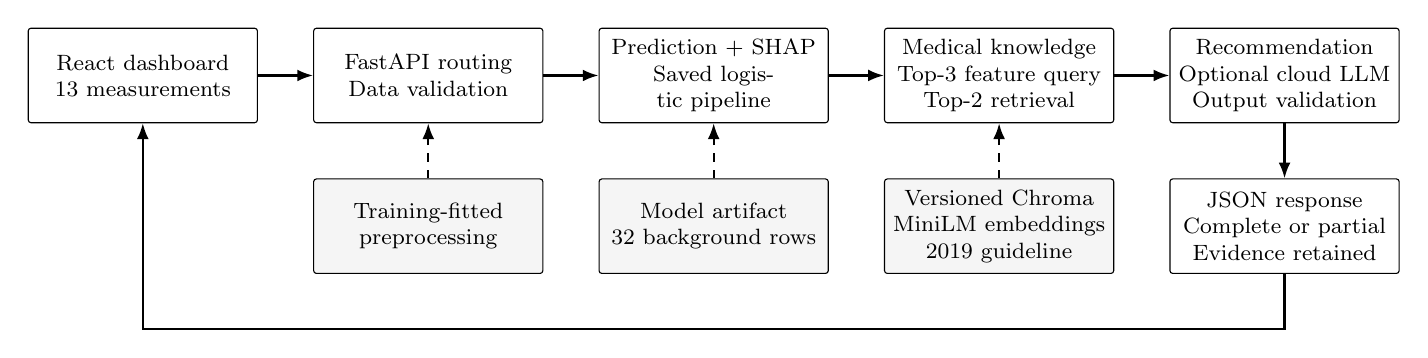
\begin{tikzpicture}[
 node distance=7mm and 7mm,
 box/.style={draw,rounded corners=1pt,align=center,font=\footnotesize,text width=27mm,minimum height=12mm,inner sep=3pt},
 artifact/.style={box,fill=black!4},
 flow/.style={-{Latex[length=2mm]},thick},
 support/.style={flow,dashed}]
\node[box] (ui) {React dashboard\\13 measurements};
\node[box,right=of ui] (api) {FastAPI routing\\Data validation};
\node[box,right=of api] (predict) {Prediction + SHAP\\Saved logistic pipeline};
\node[box,right=of predict] (rag) {Medical knowledge\\Top-3 feature query\\Top-2 retrieval};
\node[box,right=of rag] (llm) {Recommendation\\Optional cloud LLM\\Output validation};
\node[artifact,below=of api] (pre) {Training-fitted\\preprocessing};
\node[artifact,below=of predict] (model) {Model artifact\\32 background rows};
\node[artifact,below=of rag] (store) {Versioned Chroma\\MiniLM embeddings\\2019 guideline};
\node[box,below=of llm] (json) {JSON response\\Complete or partial\\Evidence retained};
\draw[flow] (ui)--(api);
\draw[flow] (api)--(predict);
\draw[flow] (predict)--(rag);
\draw[flow] (rag)--(llm);
\draw[support] (pre)--(api);
\draw[support] (model)--(predict);
\draw[support] (store)--(rag);
\draw[flow] (llm)--(json);
\draw[flow] (json.south)--++(0,-7mm)-|(ui.south);
\end{tikzpicture}

\caption{Implemented orchestration. The five responsibilities are coordinated by one FastAPI application. Solid arrows denote request dependencies; dashed arrows denote artifact or corpus inputs. The unavailable path preserves real prediction and evidence without substituting a fabricated summary.}
\label{fig:architecture}
\end{figure*}

At startup, classifier, SHAP, encoder, and retrieval components are loaded and warmed. Local inference runs in a worker thread under a single-slot semaphore, with a 0.1-second acquisition limit that returns HTTP 429 when busy. The semaphore is released before the asynchronous cloud request. Consequently, local work is serialized while cloud waits may overlap across requests. Native numerical computation is bounded to two threads.

The current synthesis provider is OpenRouter with cloud-hosted \texttt{openai/gpt-4.1-mini}; direct OpenAI remains an alternative. This configuration was introduced at commit \texttt{a9b2ac7}, after the saved evaluation snapshot. The saved timing experiment had no configured synthesis credentials and therefore contains no completed generation calls. No generator quality or live OpenRouter latency result is inferred from changing the provider. Neither Llama-3 nor Mistral is claimed as the deployed generator. No local generative LLM is hosted; MiniLM is an embedding model.

The prompt requests three sentences covering disease probability, signed contributors, and a cautious evidence-linked review point. It prohibits prescriptions, invented facts, and treating total cholesterol as LDL-C. The response validator requires exactly three bounded sentence strings, a complete provider response, and citation identifiers that match supplied evidence and the text. These checks verify output form and identifier consistency; they do not verify semantic entailment, clinical appropriateness, or factual completeness. Timeout, provider rejection, or malformed output returns a partial result with a specific reason. No cached clinical narrative is substituted.

\section{Experimental Results and Discussion}
\subsection{Protocol and Reproducibility}
The analysis uses the committed data audit, model comparison, example explanation, and integrated evaluation reports from the implementation snapshot at commit \texttt{5b3eec3}. Dataset and split checks prevent accidental changes to the held-out cohort. Model selection maximizes mean development ROC-AUC, using lower Brier score only for an exact tie. The holdout is evaluated after selection and is not used to retune the chosen model. Numerical tables and result figures in the manuscript are regenerated from these JSON reports; no additional training experiment is implied.

\subsection{Predictive Metrics and Model Comparison}
For true positives TP, true negatives TN, false positives FP, and false negatives FN,
\begin{align}
 \mathrm{Accuracy}&=\frac{\mathrm{TP+TN}}{\mathrm{TP+TN+FP+FN}},\\
 \mathrm{Precision}&=\frac{\mathrm{TP}}{\mathrm{TP+FP}},\quad
 \mathrm{Recall}=\frac{\mathrm{TP}}{\mathrm{TP+FN}},\\
 F_1&=\frac{2\mathrm{TP}}{2\mathrm{TP+FP+FN}}.
\end{align}
ROC-AUC summarizes ranking discrimination over thresholds. The Brier score,
\begin{equation}
 \mathrm{BS}=\frac{1}{n}\sum_{i=1}^{n}(p_i-y_i)^2,
\end{equation}
measures squared probability error; a favorable Brier score alone does not establish calibration across clinical subgroups.

\begin{table}[t]
\centering
\caption{Development comparison: mean over 15 folds; AUC standard deviation in parentheses.}
\label{tab:models}
\small
\begin{tabular}{lrr}
\toprule
Model & ROC-AUC (SD) & Brier \\
\midrule
Logistic ($C=0.1$) & 0.9016 (0.0391) & 0.1296 \\
Extra trees & 0.8931 (0.0419) & 0.1348 \\
Logistic ($C=1$) & 0.8924 (0.0425) & 0.1315 \\
Random forest & 0.8910 (0.0425) & 0.1351 \\
Logistic ($C=10$) & 0.8865 (0.0444) & 0.1360 \\
XGBoost & 0.8827 (0.0387) & 0.1387 \\
Calibrated RBF SVM & 0.8794 (0.0433) & 0.1385 \\
Histogram boosting & 0.8676 (0.0378) & 0.1521 \\
Prior-only dummy & 0.5000 (0.0000) & 0.2483 \\
\bottomrule
\end{tabular}
\end{table}

\begin{figure}[t]
\centering
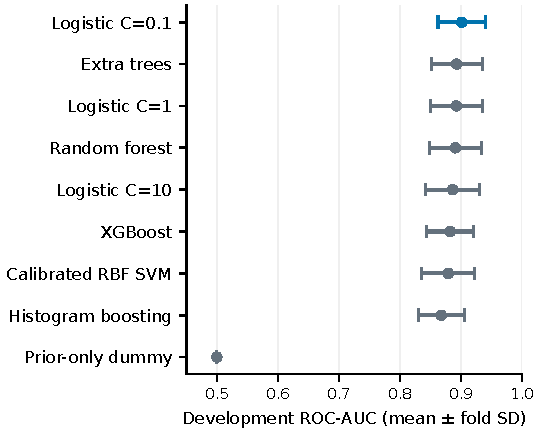
\includegraphics[width=\linewidth]{figures/results/model-comparison.pdf}
\caption{Development ROC-AUC across nine configurations. Points show means over 15 repeated stratified folds; bars show one fold standard deviation, not confidence intervals. The folds overlap.}
\label{fig:models}
\end{figure}

Table~\ref{tab:models} and Fig.~\ref{fig:models} show that logistic regression with $C=0.1$ has the highest mean development AUC, 0.9016, and the lowest Brier score, 0.1296. XGBoost achieves 0.8827 AUC under its tested configuration. Fold standard deviations describe variation among repeated validation folds; those folds overlap and are not independent trials. No statistical significance or general superiority is inferred from their ranking. The model selection process may be optimistic on development data, which is why the fixed holdout is reported separately.

\begin{table}[t]
\centering
\caption{Held-out performance of the selected logistic model ($n=61$).}
\label{tab:holdout}
\small
\begin{tabular}{lr}
\toprule
Metric & Value \\
\midrule
Accuracy & 0.8852 \\
Precision & 0.8387 \\
Recall & 0.9286 \\
F1-score & 0.8814 \\
ROC-AUC & 0.9610 \\
Brier score & 0.0869 \\
\bottomrule
\end{tabular}
\end{table}

\begin{figure*}[t]
\centering
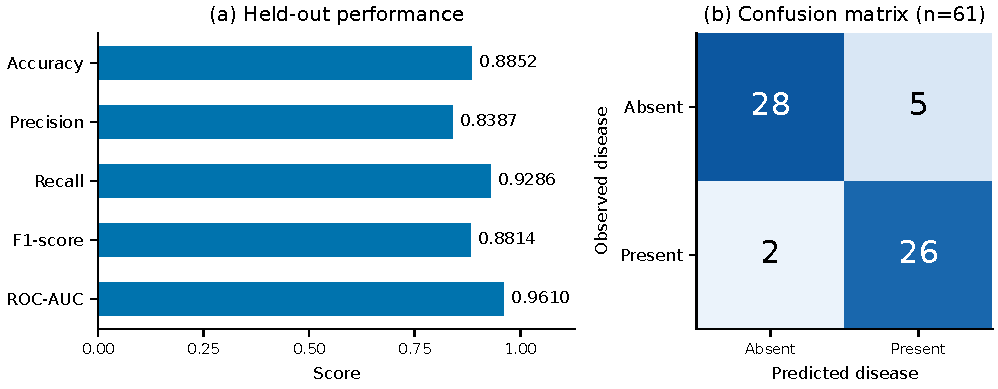
\includegraphics[width=\linewidth]{figures/results/holdout-performance.pdf}
\caption{Selected logistic model on the fixed 61-record holdout. Classification metrics use threshold 0.5; ROC-AUC uses probabilities. The confusion matrix contains raw counts (TN=28, FP=5, FN=2, TP=26).}
\label{fig:holdout}
\end{figure*}

On 61 holdout records, the selected model correctly classifies 54 cases (Table~\ref{tab:holdout}). Figure~\ref{fig:holdout} displays the measured scores and the 26 true positives, 28 true negatives, five false positives, and two false negatives. The 1,000-resample percentile bootstrap ROC-AUC interval is approximately [0.9021, 0.9989]. This descriptive interval is conditional on a small holdout, not a measure of external transportability. The higher holdout AUC relative to development AUC should not be interpreted as a robust improvement; sampling variation is substantial at this scale.

No prospective, temporal, multicenter, or subgroup fairness validation is available. Demographic distributions and diagnostic-test availability may differ markedly in deployment. Accuracy on this cohort therefore cannot establish safe screening, prognosis, or treatment selection. In particular, outcome prevalence and the 0.5 classification threshold have not been chosen for a clinical decision pathway.

\subsection{Retrieval Quality}
Let $R_k(q)$ be the unique retrieved identifiers within $k$ returned slots and $G(q)$ the labeled relevant set. The evaluation definitions are
\begin{equation}
 P@k=\frac{|R_k(q)\cap G(q)|}{k},\qquad
 R@k=\frac{|R_k(q)\cap G(q)|}{|G(q)|}.
\end{equation}
Missing or duplicate hits receive no additional credit. Precision@2 is recorded in the evaluation report. Recall@2 in Table~\ref{tab:retrieval} is computed for this manuscript from the same stored retrieved and relevant identifiers, without executing a new retrieval experiment.

\begin{table}[t]
\centering
\caption{Development retrieval diagnostic. Recall is relative to the recorded seed labels.}
\label{tab:retrieval}
\small
\begin{tabular}{lrrr}
\toprule
Topic & $|G|$ & P@2 & R@2 \\
\midrule
Physical activity & 3 & 1.0000 & 0.6667 \\
Aspirin: age over 70 & 1 & 0.0000 & 0.0000 \\
Aspirin: bleeding risk & 2 & 1.0000 & 1.0000 \\
Dietary pattern & 4 & 0.0000 & 0.0000 \\
Obesity / weight loss & 4 & 1.0000 & 0.5000 \\
LDL-C $\geq190$ mg/dL & 1 & 0.5000 & 1.0000 \\
Mean & -- & 0.5833 & 0.5278 \\
\bottomrule
\end{tabular}
\end{table}

\begin{figure}[t]
\centering
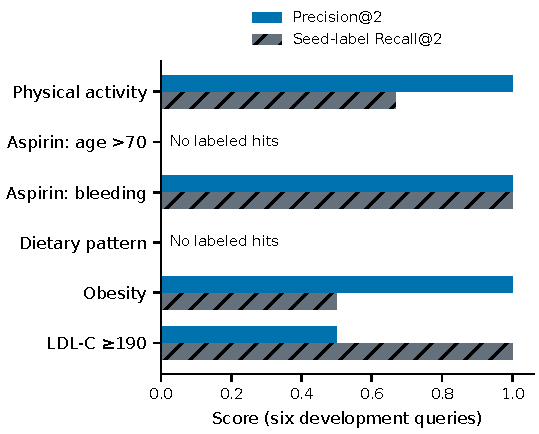
\includegraphics[width=\linewidth]{figures/results/retrieval-quality.pdf}
\caption{Retrieval diagnostics for six development queries. Recall uses the stored seed-label set, not exhaustive clinical relevance judgments. Zero-hit topics remain visible.}
\label{fig:retrieval}
\end{figure}

As shown in Fig.~\ref{fig:retrieval}, the six queries yield mean Precision@2 of 0.5833 and mean labeled-set Recall@2 of 0.5278. These are implementation-time, source-grounded seed judgments, not independent clinician annotations or an exhaustive relevance assessment. A singleton labeled set cannot exceed Precision@2 of 0.5. Consequently, unlabeled relevant passages can be counted as nonrelevant, and the recall values quantify recovery of the recorded labels rather than comprehensive clinical evidence coverage.

The age-specific aspirin query and dietary-pattern query retrieve no labeled relevant passages. In particular, the aspirin-over-70 query misses the explicit age-qualified warning. That failure illustrates why citation availability must not be conflated with evidence adequacy. Retrieval can find topically related context while failing to preserve the qualifier that determines relevance. The manual diagnostic queries also differ from actual SHAP-derived queries; they do not establish the latter's accuracy across the patient cohort. Corpus filtering and query development occurred during implementation, so these measurements are development diagnostics rather than an unbiased benchmark.

\subsection{Latency and Operational Behavior}
The critical path can be expressed as
\begin{equation}
\begin{split}
 T_{\mathrm{total}}={}&T_{\mathrm{validation}}+T_{\mathrm{queue}}
 +T_{\mathrm{prediction+SHAP}}\\
 &+T_{\mathrm{retrieval}}+T_{\mathrm{cloud}}+T_{\mathrm{serialization}}.
\end{split}
\end{equation}
The saved classifier-only warm prediction median is 2.46 ms over thirty calls. This excludes SHAP, retrieval, HTTP, and cloud generation. Ten recorded local HTTP requests complete with real model output and retrieved passages, but all report \texttt{provider\_not\_configured}. Their partial-response median is 62.56 ms. Complete synthesis succeeds in zero of ten requests; complete-response median and 95th-percentile latency are therefore unmeasured. The under-three-second full-pipeline target is not demonstrated.


\begin{figure}[t]
\centering
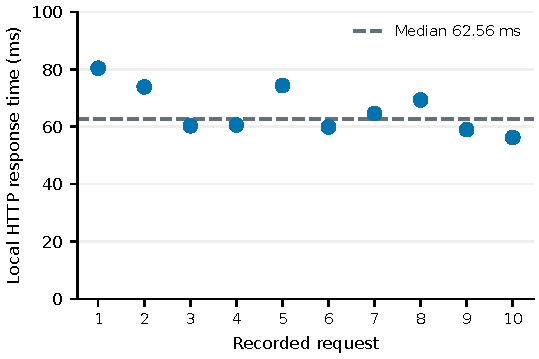
\includegraphics[width=\linewidth]{figures/results/partial-latency.pdf}
\caption{Ten recorded partial HTTP responses; every request lacked a configured synthesis provider. The dashed line is the median. These are not complete cloud synthesis latencies.}
\label{fig:latency}
\end{figure}
Figure~\ref{fig:latency} shows every recorded partial response. These timings describe warm local research execution, not throughput under load. Hardware was not comprehensively recorded in the evaluation artifact, so the observations should not be treated as a hardware-independent benchmark. Provider network latency, generation time, cold startup, concurrency, and failure recovery require separate measurement. Bounded timeouts constrain waiting but cannot establish acceptable clinical workflow latency.

\subsection{Interpretability, Safety, and Threats to Validity}
The saved synthetic example has disease probability 0.8389 and baseline probability 0.4148. Its strongest recorded positive contributions are thallium result (+13.15 percentage points), chest-pain type (+8.06), and exercise-induced angina (+6.27). These are explanations of one artificial input, not findings about a treated patient. They illustrate the interface's intended inspection path: read the estimate, examine signed contributors, then verify the retrieved source.


\begin{figure}[t]
\centering
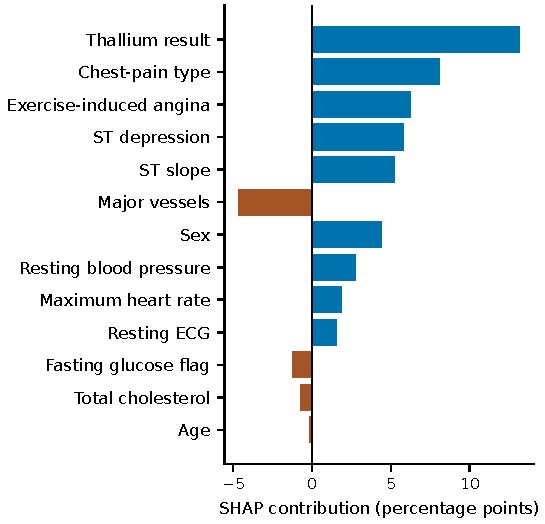
\includegraphics[width=\linewidth]{figures/results/local-shap.pdf}
\caption{Original-feature permutation SHAP for one synthetic input. Contributions are in probability percentage points; baseline 41.48\% plus all signed contributions gives 83.89\%. Positive bars increase the model output; negative bars decrease it. This is not a patient outcome or causal effect.}
\label{fig:shap}
\end{figure}
Figure~\ref{fig:shap} includes all thirteen signed contributions rather than only the three used to form the retrieval query. This design may make model behavior easier to inspect, but no clinician study measures understanding, trust calibration, reading time, or decision quality. Likewise, no factuality annotation or controlled generator comparison measures hallucination reduction. Assertions that agent decomposition improves diagnostic accuracy or lowers hallucination rates would exceed the evidence. The demonstrated benefit is traceability of intermediate outputs and explicit handling of incomplete execution.

The numerical model and corpus also target different clinical contexts. Total cholesterol is not LDL-C, elevated fasting glucose is not a confirmed diabetes diagnosis, and a Cleveland disease-presence probability cannot replace a ten-year ASCVD estimate. Two short passages can omit contraindications, exceptions, or adjacent table definitions. Extraction artifacts may fragment tables, and valid citation identifiers do not ensure that the cited text supports the generated claim. The prototype has no production authentication, EHR integration, or prospective governance evaluation. Cloud use requires an appropriate data-sharing and consent framework; a public research dataset does not authorize transmission of future identifiable patient data.

\section{Conclusion and Future Works}
\system{} implements a full-stack research framework that connects a selected cardiovascular classifier to original-feature explanations, provenance-preserving guideline retrieval, and optional constrained synthesis. The selected logistic model attains 88.52\% holdout accuracy and 0.9610 ROC-AUC under a fixed small-cohort protocol. Retrieval diagnostics expose clinically important gaps, while explicit partial responses prevent absent cloud generation from being presented as successful synthesis. The central contribution is an inspectable integration of responsibilities rather than a demonstrated improvement in patient outcomes.

Several limitations follow directly from the implementation. Dependent prediction, explanation, retrieval, and synthesis stages accumulate latency; they are not parallelized merely by naming them agents. Only the final generator is a remote service in the present design, so multiple sequential inter-agent network calls are a potential future cost rather than a measured current behavior. Local LLM hosting would introduce memory, compute, energy, and maintenance expense, but those costs are not measured here because generation is cloud-hosted. Evidence quality is strictly bounded by the embedded source, extraction fidelity, chunking, and retrieval relevance. A static 2019 corpus cannot represent automatically current medical guidance.

Future work should prioritize external predictive validation, independent relevance annotation, and end-to-end factuality assessment before increasing architectural complexity. Retrieval improvements should test qualifier-aware queries, hybrid search, reranking, and expanded context using held-out clinical questions. A controlled reader study should compare probability-only, probability-plus-SHAP, and evidence-grounded interfaces. Generator evaluation should measure unsupported claims and citation entailment against an ungrounded baseline while reporting complete-call latency and cost.

Multimodal extensions could incorporate imaging or physiological signals, provided modality-specific validation and attribution are added. Real-time EHR integration would require interoperable data mapping, access control, consent, auditability, and monitoring for distribution shift. These extensions should preserve the present separation between observed measurements, model-derived associations, retrieved statements, and human clinical judgment.

\bibliographystyle{IEEEtran}
\bibliography{references}
\end{document}
